\chapter{Implementation}
\label{chapter:Chapter 4}

\section{JavaScript Performance}

The first problem in implementing a game engine in JavaScript will be the performance problem caused by the fact that it’s a interpreted and garbage collected language. Modern JavaScript engine implementations try to address this by using a Just in Time (JIT) compiler.

\subsection{Strict mode}

Having a JIT is not enough, as vanilla JavaScript allows you to do a lot of operations which can not be optimized by a JIT, like accessing the callee of a function and its properties. This behavior is not JIT-able as the reference to the callee depends on the context in which the function is called. This made the standardization committee to implement a strict mode in ECMAScript 5. The strict mode is just specifying that the current scope is written in a subset of JavaScript that can be easily compiled and does not have undefined behavior. Strict mode also brings a less error prone coding to JavaScript, one of these features is that variables must be explicitly declared before using them, as opposed to normal JavaScript, when if you use a variable which is not declared it will automatically declare it in the global scope.

\subsection{AsmJS mode}

AsmJS mode is a special mode created by Mozilla and implemented in Firefox. The AsmJS subset of JavaScript can be compiled Ahead of Time (AOT) and it has a stack based memory model. All the variables must be typed. In order for the AsmJS subset to be compatible with engines that don’t know how to interpret it all, the operations that specify type must be no-ops. The only two types supported in AsmJS are “double” and “int”. In order to say that a variable is an “int”, it needs to be bitwise or with 0 (e.g. x = x|0). For “double”, it needs to have a attribution with his sign explicitly defined (e.g. x = +x). This allows for AsmJS to conform to the JavaScript standard.

\subsection{Memory model}

JavaScript is a garbage collected language. All the variables in JavaScript are prototypes which means that they are objects, but for performance reasons various JavaScript engine’s implement Just In Time compilers (JITs) that can compile a certain subset of JavaScript into native code. Some of the JITs have special optimizations for certain variable uses. For example, Chrome’s V8 has optimization for arrays (variables which have the prototype as the Array object), that translates them to normal arrays, but only as long as no other property is attached to it. If this happens, then it falls back to lesser optimized implementations. Arrays by their nature, in JavaScript are just a special case of an object which inherits the Array object. Thus, inherits its methods and properties, but each index can also be accessed by referencing to it in a property way (i. e. array.1 instead of array[1]). This coupled together with the fact that you can also access properties through the [] operator (i.e. array[‘length’] instead of array.length), can lead to the creation of sparse arrays. Sparse arrays aren’t optimized in the JIT as demonstrated in V8 (from reference \cite{clifford12}).

Another problem that JavaScript poses is the fact that all of its arithmetic and numbers are stored on double precision floating point numbers. This makes some of the calculations more slower than expected. It can also introduce type incompatibilities, so in order to interface with WebGL, we need to use TypedArrays. A TypedArray has a backing ArrayBuffer which is a contiguous memory zone. It offers an array like API with a backing store of 8 bit unsigned integers. A TypedArray is just a higher level view of an underlying part of an ArrayBuffer, taking care of implementing arrays of different types over the ArrayBuffer. The types implemented are: Int8Array, Uint8Array, Int16Array, Uint16Array, Int32Array, Uint32Array, Float32Array, Float64Array. Due to the fact that  JavaScript is still a garbage collected language, this means that although we can allocate these buffers, we can’t also discard of them when they are of no more use.

In Game Engine Architecture \cite{gregory09}, it is presented that most game engines implement their own memory management by preallocating a large buffer and then writing their own allocation routines. One of the simpler routines presented is the stack like allocation, in which a stack pointer is moved with each allocation.

A implementation of a similar allocator in JavaScript can be found in the listing ~\ref{lst:allocation-benchmark}

\lstset{caption=Allocation benchmark (allocator.js), label=lst:allocation-benchmark}
\lstinputlisting{src/listings/allocator.js}

The most called out size for a TypedArray allocation is 16 as this is the size of a 4x4 matrix used for transformations. Another allocation size is around 10000 which can be the average size of a vertex buffer or an index buffer. To top it up, a larger allocation size can be around tens of MB of RAM, which can represent textures. I am going to use these three dimensions in a allocation benchmark\footnote{http://jsperf.com/allocator-test/2, accessed on 10.09.2014} in order to test how much gain the engine can get from using a custom allocator.

\begin{center}
	\begin{figure}[here!]
		
		\includegraphics[width=\textwidth]{src/img/chart1.png}
		\caption{Benchmark Allocation}
		\label{img:chart1}
	\end{figure}
\end{center}

As can be seen from the benchmark results (~\ref{img:chart1}), there is no increase in performance by implementing a custom allocator for JavaScript. The only size for which an increase in performance is seen is for a allocation size of 1000. This is quite peculiar, as it would have been expected to see an increase in performance for the case in which a small array is allocated, like for size 16.

\subsection{Speed}

In order to compare if AsmJS offers any speed improvements for raw processing power, I've looked at a couple of benchmarks.

The first benchmark\footnote{http://jsperf.com/slow-asm-js/4, accessed on 10.09.2014} compares two identical murmur3 hash implementations: one using AsmJS and one not using AsmJS. 
As it can be seen in figure ~\ref{img:murmur3}, AsmJS doesn't bring any optimizations to the bitwise operations done by Murmur3 Hash.
\begin{center}
	\begin{figure}[here!]
		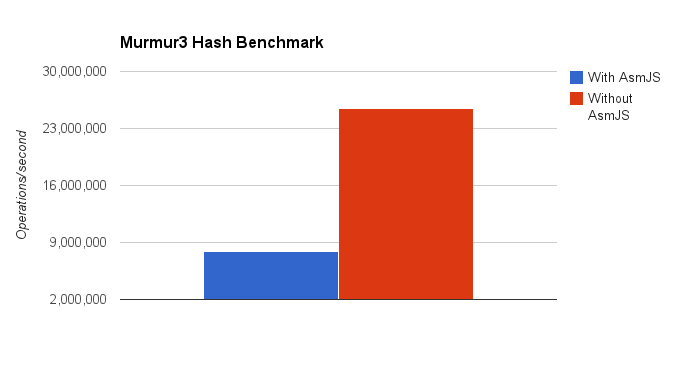
\includegraphics[width=\textwidth]{src/img/murmur3.png}
		\caption{Benchmark Murmur3}
		\label{img:murmur3}
	\end{figure}
\end{center}
In our days compilers have different levels of optimizations available, one of the options most compilers have is loop unrolling for fixed size small loops. In the following benchmark\footnote{http://jsperf.com/matrix-multiplication-with-asm-js/6, accessed on 10.09.2014}, I am testing to see if the JavaScript JIT or AOT will perform this kinds of optimizations.
As it can be seen from the benchmark results ~\ref{img:matrix-mul}, the compiler does not do any loop unrolling.
\begin{center}
	\begin{figure}[here!]
		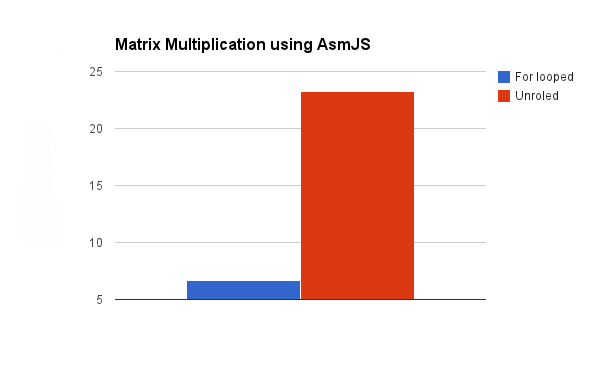
\includegraphics[width=\textwidth]{src/img/matrix-mult.png}
		\caption{Matrix Multiplication Benchmark}
		\label{img:matrix-mul}
	\end{figure}
\end{center}

\FloatBarrier
\section{Engine architecture}

The engine is made out of different modules. Each module needs some other modules in order to function. Each of these modules offer an API which they must respect in order for them to function properly, for example the rendering module offers an API which helps rendering. You can replace the rendering module with your own rendering module but you need to respect its API in order for the engine to function. This can be implemented in Java using Interfaces, but since JavaScript doesn’t offer such a feature, nor does it offer a replacement for abstract classes, you can’t force a module to implement an API.

The modules that represent the engine are:
\begin{easylist}[itemize]
& Rendering
& Input Control
& Resource Manager
& Camera
& Physics Engine
& Scripting
& Timer
& Audio Manager
\end{easylist}
\section{Asset Pipeline}

In order to import assets into a game engine, all the major engines require an asset pipeline that pre-processes assets. This engine is not different from the others. Because asset importing takes a lot of parsing and processing, it is best to be done offline. In the engine, the asset pipeline consists in using assimp2json in order to convert the files to the same format. If there are more modifications needed to be done on the file, then the file can be modified using a simple text editor. All the assets are grouped in zip files. Each corresponding zip file corresponds to a portion of game data that must be loaded at runtime all at once, like all the data necessary for a game level. It must also contain a manifest file. This manifest file specifies options regarding the loaded data file like: paths or various types of files, the main scene file to load. These are specified in a file named manifest.json.

\section{Resource Manager}

The resource manager takes care of downloading and storing the resources. It uses zipjs in order to read the data files. Zipjs offers a virtual file system that can be used in order to load files from the game data archive.
The resource manager is responsible for loading the data and the scene from the file system. It parses the scene files and creates scene objects from them. It does a preloading of all the scenes in the file, so that if a scene references another scene inside itself it should be already loaded. It also handles texture loading from files and replaces them with image objects which can be used to load textures onto objects.

\section{Rendering Engine}

The rendering engine is a replaceable part of the game engine. It was written specifically so that it can easily be replaced with another rendering engine if necessary.
The implemented rendering engine uses the deferred rendering technique. It has a G-Buffer inspired from the Killzone 2’s G-Buffer without the render targets for motion blur.
It uses the WEBGL\_draw\_buffers extension in order to bind multiple render targets to a frame buffer. The WEBGL\_draw\_buffers extension has the same limitation as on last generation consoles, just four render targets plus the twenty four bit depth buffer with eight bit stencil buffer texture and only 8 bit per color textures.
In order to get the world position of each fragment, the depth texture is sampled and converted into view space coordinates.

Depth can be saved in two ways: either using the UNSIGNED\_INT\_24\_8\_WEBGL depth texture or by saving the depth in a 32 bit using a RGBA8 texture.
In order to save the depth into the RGBA8 texture, it needs to be packed. For that, I am using the functions (specified in \cite{engel14}) which you can see in listing \ref{lst:packing}.

\lstset{caption=RGBA8 packing, label=lst:packing}
\lstinputlisting{src/listings/pack.fs}

The depth buffer, after multiplying it with the reverse projection matrix, looks like in figure ~\ref{img:depth}.
From that depth buffer, I multiply it with the view matrix to obtain the view space position, a rendering of the scene with the view space coordinates encoded into the RGB values can be found at figure ~\ref{img:view-space}.

\section{Input Control}

The input control system handles all the bindings to the DOM events. Then, it forwards the events to the current InputControl object. 
Each InputControl object holds an ArrayBuffer which contains the state of the keys. The input control is based on actions, each action is defined by a set of keys which can trigger it. The set of keys is defined as a string representing them. Each of these keys pressed is enough to consider the action to be true. One of this sets is named an action. In order to check if an action is true, the API offers an action method which needs to be called using the name of the action. There can be multiple input controls defined, but only one active at a certain time. Activating an input control is done by using the useInputControl method. 

HTML5 had an API which allows mouse locking to occur, named PointerLock API. Each time we request a pointer lock, this triggers a visual confirmation prompt to the user who must allow or deny the pointer lock. This is different from the usual desktop implementation which doesn't require confirmation from the user in order to lock the mouse pointer.
The API also offers the possibility to receive mouse moves as a delta from the last mouse move event. The drawback of using this API is that it binds the ESC key to itself in order to allow the user to exit the mouse lock. 


\section{Camera}

The camera system handles the view and projection matrices. Each camera must implement its own way of handling these. Each camera is also offered access to the input system in order for camera movement to be possible. 

The implemented camera is a orbiting perspective camera. It holds its angle in a quaternion. This is done in order to maintain the possibility of doing affine transformations on the camera position and rotation. The camera is responsible for updating the renderer’s view and projection matrices.

The camera system handles multiple camera types:
\begin{easylist}
& Scene based camera
& Random camera
\end{easylist}

A scene based camera is part of the scene graph and has a parent and possibly children attached to it. Its position is calculated based on the position of the parent. It has the same properties as any other object in the scene graph, it too can have for example a physics object attached to it, it can also have scripting attached to it. It is extremely useful for creating 3rd person cameras that need to have collision shapes.

Random cameras are cameras that extend the $Camera$ class and implement their own behavior. For example, the implemented orbiting camera is such a camera because it orbits around the center of the scene and is not part of the scene. 

\section{Physics Engine}

The physics engine is just a wrapper over Ammo.JS. The wrapper is necessary in order to execute the physics engine on another thread using web workers.
Each node on the scene graph has a physics properties object which is linked to the physics object simulations. The scene graph is sent to the physics worker between each frame. The physics worker parses the scene graph and updates the physics properties of the objects according to the physics simulation.

AmmoJS uses Bullet physics engine to do the physics simulation, itself is just a wrapper over Bullet's methods, for example in order to call $btDefaultCollisionConfiguration$ we call it using AmmoJS via its wrapper class Ammo, $Ammo.btDefaultCollisionConfiguration$.

Due to the fact that this is Emscripten compiled code, one must be careful to deallocate objects that it creates, since all the objects created are allocated on the same ArrayBuffer that is used as a heap zone so JavaScript's garbage collector can't collect them. In order to deallocate an object we must call it's $destroy$ method.
\section{Scripting}

The scripting system is based upon the fact that JavaScript is an interpreted language. All the scripts are wrapped in a JavaScript scope, where a couple of objects are made available. The scope is created by inserting the JavaScript code into a function body. This can be done because in JavaScript functions are first-class citizens, this means that functions can be manipulated however the programmer wants. Of course this does not allow the JIT to compile something that might modify itself, so under strict mode only the creation of new functions is possible. This can be done using the Function prototype.
The only problem with this model is that inclusion of other scripts is not possible, which lead to including a lot of objects into the scope of the script.
These objects are:

\begin{easylist}[itemize]
& Scene graph - the current scene graph object is included in order for the script to be able to manipulate the scene’s objects. This scene graph also contains the physics objects used to calculate the object’s physics.
& Global storage - an object which can be used by the scripts in order to be able to store data between executions.
& Resource manager - the resource manager is present here in order to be able to load different scenes or different game data files, like for example a new level.
& Math helper classes - classes like mat4, vec3 and all the other classes that the gl-matrix library offers are passed into the scope in order for scripts to be able to do mathematical operations easier
& Timer system
& Audio Manager
\end{easylist}
You might notice that no persistent storage is offered. This is done because the scripts already have access to persistent storage by using the normal browser API’s like IndexedDB or LocalStorage. These should be sufficient for all the script’s needs.
Due to the fact that JavaScript is run on a single thread, it is possible for scripts to run for a longer duration without the possibility to stop their execution. This can be solved by executing them in a SharedWorker, but this means that all these objects need to be passed each time the script is executed, which might have a negative impact on the engine’s performance.
Another popular scripting language is Lua. Lua can be run from JavaScript using Moonshine, a Lua VM written in JavaScript. 
C++ scripting can also be integrated by compiling the scripts using Emscripten, but because of Emscripten’s bootstrapping for each C++ code, it is probably not preferred.

Since scripts are run on the rendering thread it is possible for them to call out globally implemented code and bind into other JavaScript scripts or browser APIs.
\section{Timer}

The timer module is a utility module that gives the programmer all the timing option he needs. In order to offer high precision timing, the timer module uses the high precision time function: window.performance.now(). This function is useful for implementing high resolution timers.
The most basic timers are profiling timers. These are used to track and aggregate stats regarding a certain operation that the programmer wants profiled. It keeps track of subsequent invocations of the same timer id and generates the minimum time interval, the maximum time interval and the average time interval for each timing. It can print a report of all the timers. You can use the profiling feature by calling the start and stop methods of the Timer class. These methods take a single parameter: the id of the profiled section. The id should be mapped to a name using the map method; this ensures that the timer is presented in the statistics.

Another type of timers are real time timers. These timers track the time passing in real time. They are useful for interpolating animations and various other effects. These timers are instanced based. They are obtained by instantiating a RealTimeTimer object.

The last type of timers are discrete timers. Discrete timers are obtained by calling the getTimer method of a DiscreteTimeClock. The discrete timer measures the time passed from the creation of the object to the current time of the discrete clock it’s associated with.

\section{GUI}

Because the WebGL context is rendered in a canvas element inside a HTML5 web page, any normal HTML element can be overlayed on top of the canvas area to create a GUI (Graphical User Interface).
Using CSS3 3D transforms, HTML elements can be used in order to create a immersive HUD (Head-Up Display) for the game that is overlayed on top of the rendering canvas.
This has multiple advantages:
\begin{easylist}[itemize]
& Support for a variety of fonts and fast text rendering.
& Event based GUI elements
& Use of the same language (JavaScript) for GUI and for the engine.
& Simple language for creating GUI elements (HTML)
& Hardware accelerated special effects (CSS3 transforms)
& Easy social media integration (through available APIs for web pages)
& Easy integration with other online resources (you can include another webpage using an iframe).
\end{easylist}       

Another advantage of implementing a GUI in HTML5 is leveraging the video element. The video element can playback any format of video stream that the browser supports which currently are:
\begin{easylist}
& VP8
& VP9
& Theora
& H.264
\end{easylist}

The advantage is that for some formats like H.264 browsers already use hardware acceleration out of the box\footnote{https://bugzilla.mozilla.org/show_bug.cgi?id=714408} on multiple platforms including mobile devices.
\section{Audio Manager}
The audio manager leverages the HTML5 Audio API in order to handle the playback of media files. The files must be loaded from the game data virtual filesystem. The audio manager uses the resource manager in order to load the audio file into an ArrayBuffer object. Afterwards from it it creates a AudioBuffer which it can then manipulate. 

The audio API can play any type of file that can be supported by the browser.
According to Mozilla Developer Network \footnote{https://developer.mozilla.org/en-US/docs/Web/HTML/Supported_media_formats} the supported media formats are:
\begin{easylist}
& Wave
& WebM
& MP3
& AAC
& Opus
\end{easylist}

The number of simultaneous audio streams played is dependent on the implementation of the browser. For example, Safari on iOS can only play one audio file at a time\footnote{https://developer.apple.com/library/safari/documentation/audiovideo/conceptual/using_html5_audio_video/device-specificconsiderations/device-specificconsiderations.html}.